%%%%%%%%%%%%%%%%%%%%%%%%%%%%%%%%%%%%
% Slide options
%%%%%%%%%%%%%%%%%%%%%%%%%%%%%%%%%%%%

% Option 1: Slides with solutions

\documentclass[slidestop,compress,mathserif]{beamer}
\newcommand{\soln}[1]{\textit{#1}}
\newcommand{\solnGr}[1]{#1}

% Option 2: Handouts without solutions

%\documentclass[11pt,containsverbatim,handout]{beamer}
%\usepackage{pgfpages}
%\pgfpagesuselayout{4 on 1}[letterpaper,landscape,border shrink=5mm]
%\newcommand{\soln}[1]{ }
%\newcommand{\solnGr}{ }

%%%%%%%%%%%%%%%%%%%%%%%%%%%%%%%%%%%%
% Style
%%%%%%%%%%%%%%%%%%%%%%%%%%%%%%%%%%%%

\def\chp7@path{../../Chp 7}
\input{../../lec_style.tex}


%%%%%%%%%%%%%%%%%%%%%%%%%%%%%%%%%%%%
% Preamble
%%%%%%%%%%%%%%%%%%%%%%%%%%%%%%%%%%%%

\title[Lecture 28]{MA213: Lecture 28}
\subtitle{Module 4: Inference}
\author{OpenIntro Statistics, 4th Edition}
\institute{$\:$ \\ {\footnotesize Based on slides developed by Mine \c{C}etinkaya-Rundel of OpenIntro. \\
The slides may be copied, edited, and/or shared via the \webLink{http://creativecommons.org/licenses/by-sa/3.0/us/}{CC BY-SA license.} \\
Some images may be included under fair use guidelines (educational purposes).}}
\date{}


%%%%%%%%%%%%%%%%%%%%%%%%%%%%%%%%%%%%
% Begin document
%%%%%%%%%%%%%%%%%%%%%%%%%%%%%%%%%%%%

\begin{document}


%%%%%%%%%%%%%%%%%%%%%%%%%%%%%%%%%%%%
% Title page
%%%%%%%%%%%%%%%%%%%%%%%%%%%%%%%%%%%%

{
\addtocounter{framenumber}{-1} 
{\removepagenumbers 
\usebackgroundtemplate{\includegraphics[width=\paperwidth]{../../OpenIntro_Grid_4_3-01.jpg}}
\begin{frame}

\hfill \includegraphics[width=20mm]{../../oiLogo_highres}

\titlepage

\end{frame}
}
}


%%%%%%%%%%%%%%%%%%%%%%%%%%%%%%%%%%%%
% Recap/Agenda 
%%%%%%%%%%%%%%%%%%%%%%%%%%%%%%%%%%%%
% TODO better formatting
\begin{frame}
    \frametitle{Module 4: Inference}
    \begin{itemize}
        \item \hl{Previously: }Power calculations for a difference of means (Chapter 7.4)
        \item \hl{This time: } Issues with Hypothesis Testing 1: The traps of insufficient power
        \item \hl{Reading: }Chapter 7.5 for next time
        \item \hl{Deadlines/Announcements: }
    \end{itemize}
    
\end{frame}
%%%%%%%%%%%%%%%%%%%%%%%%%%%%%%%%%%%%
% Sections
%%%%%%%%%%%%%%%%%%%%%%%%%%%%%%%%%%%%

%%%%%%%%%%%%%%%%%%%%%%%%%%%%%%%%%%%%

\begin{frame}
\frametitle{Reminder: Power}
  \begin{center}
      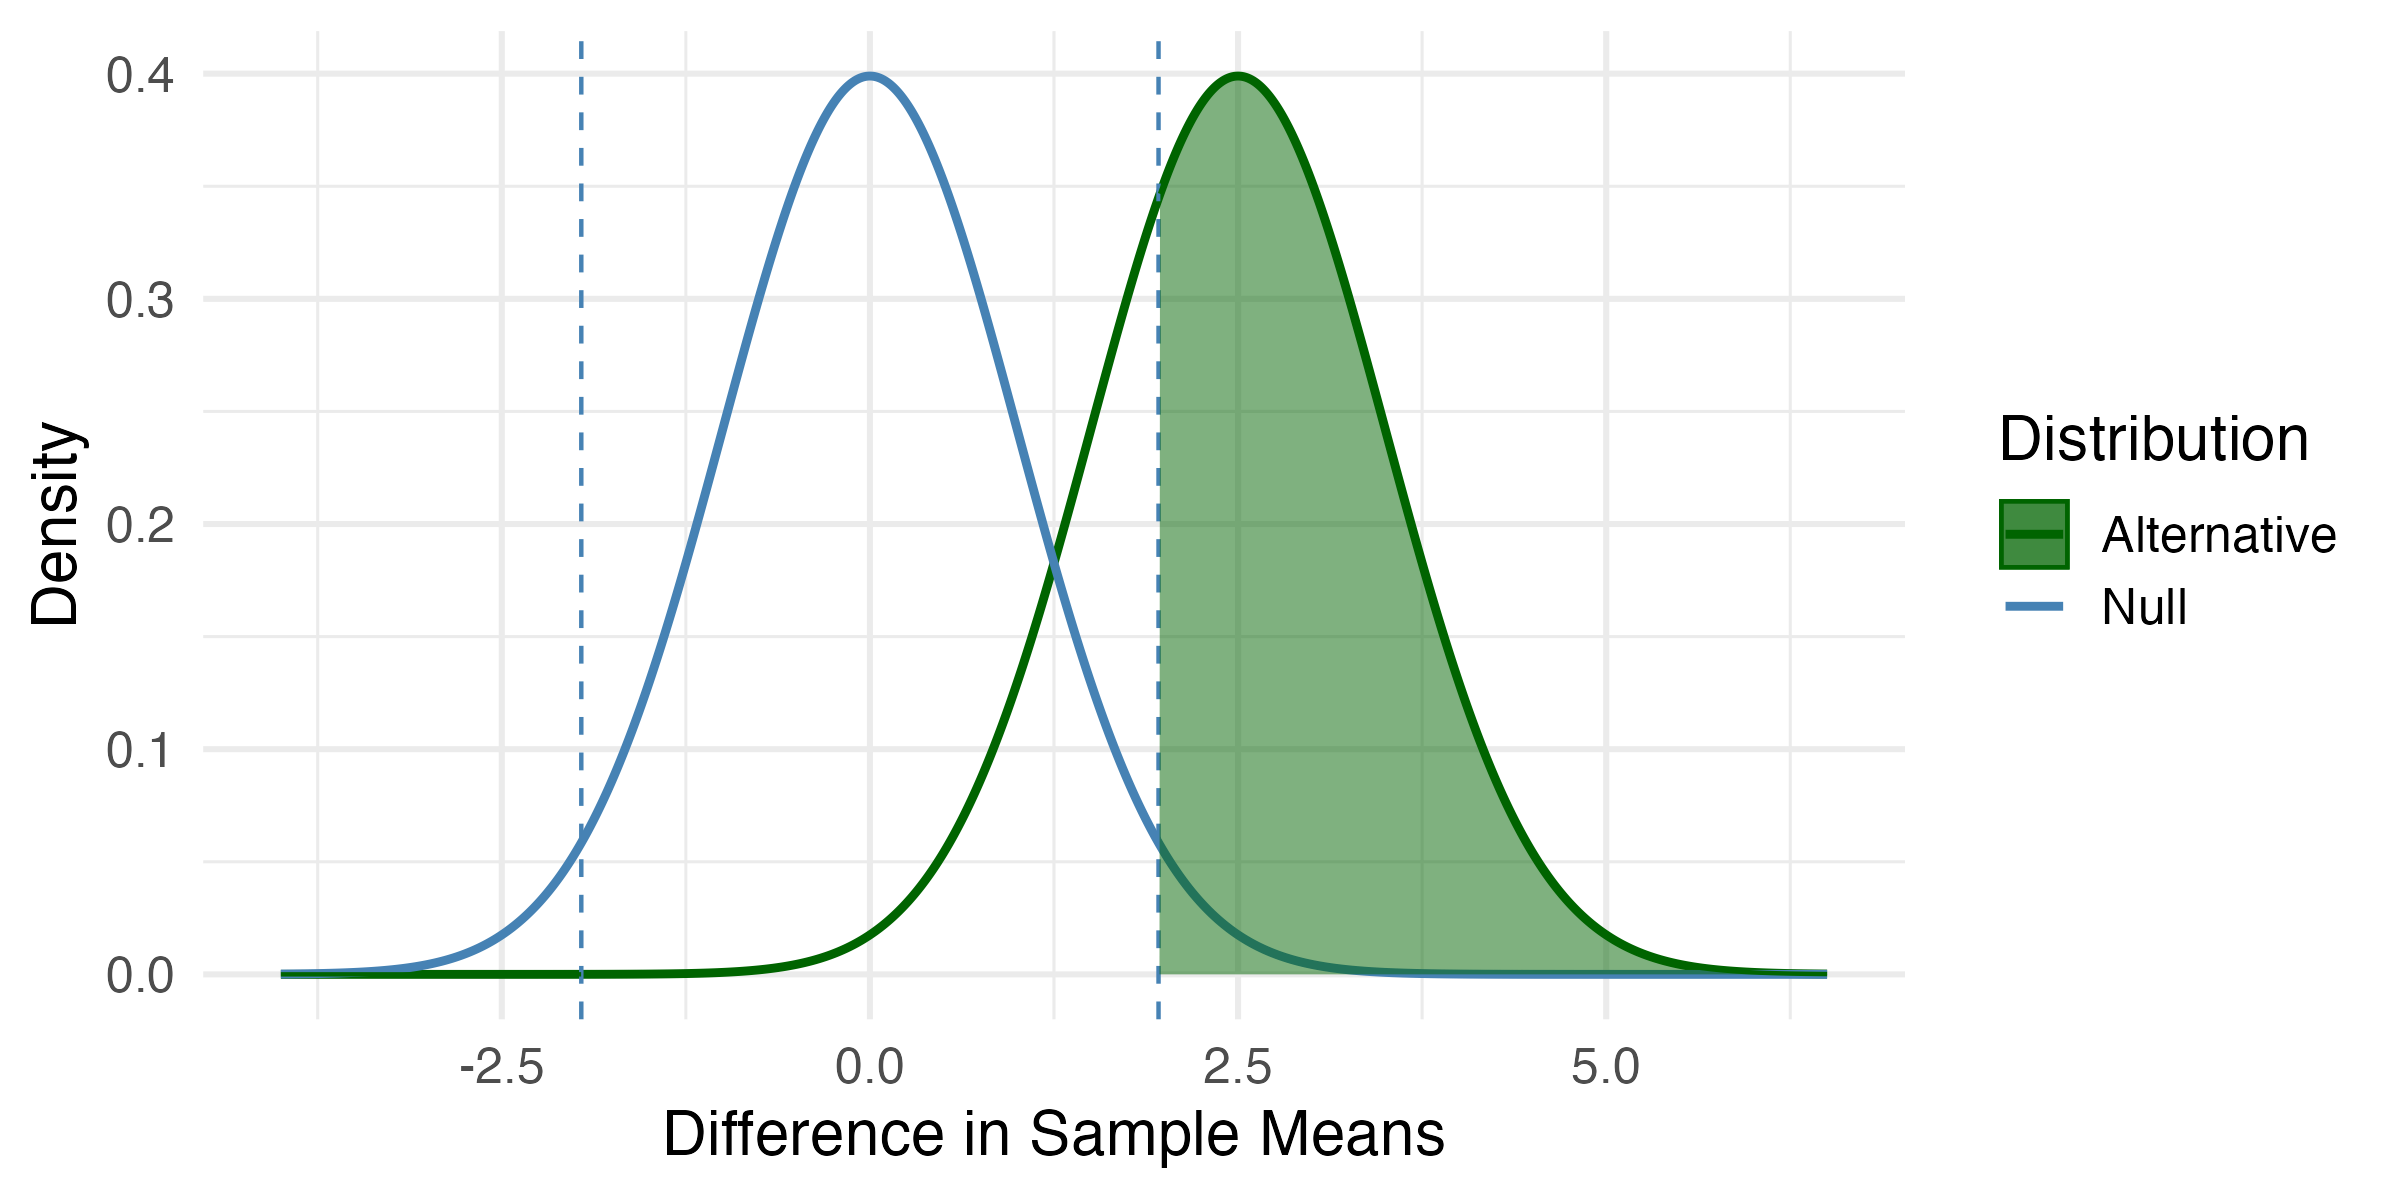
\includegraphics[width=\textwidth]{../Lecture27/figures/whatif_baseline.png}
  \end{center}
  What if the effect size is very low?
\end{frame}

%%%%%%%%%%%%%%%%%%%%%%%%%%%%%%%%%%%%

\section{R demo: (Shiny App) What if the effect size is very low?}
\section{Edfinity Quiz: What if the effect size is very low?}

%%%%%%%%%%%%%%%%%%%%%%%%%%%%%%%%%%%%

\begin{frame}
\frametitle{What if the effect size is very low?}
  \begin{center}
      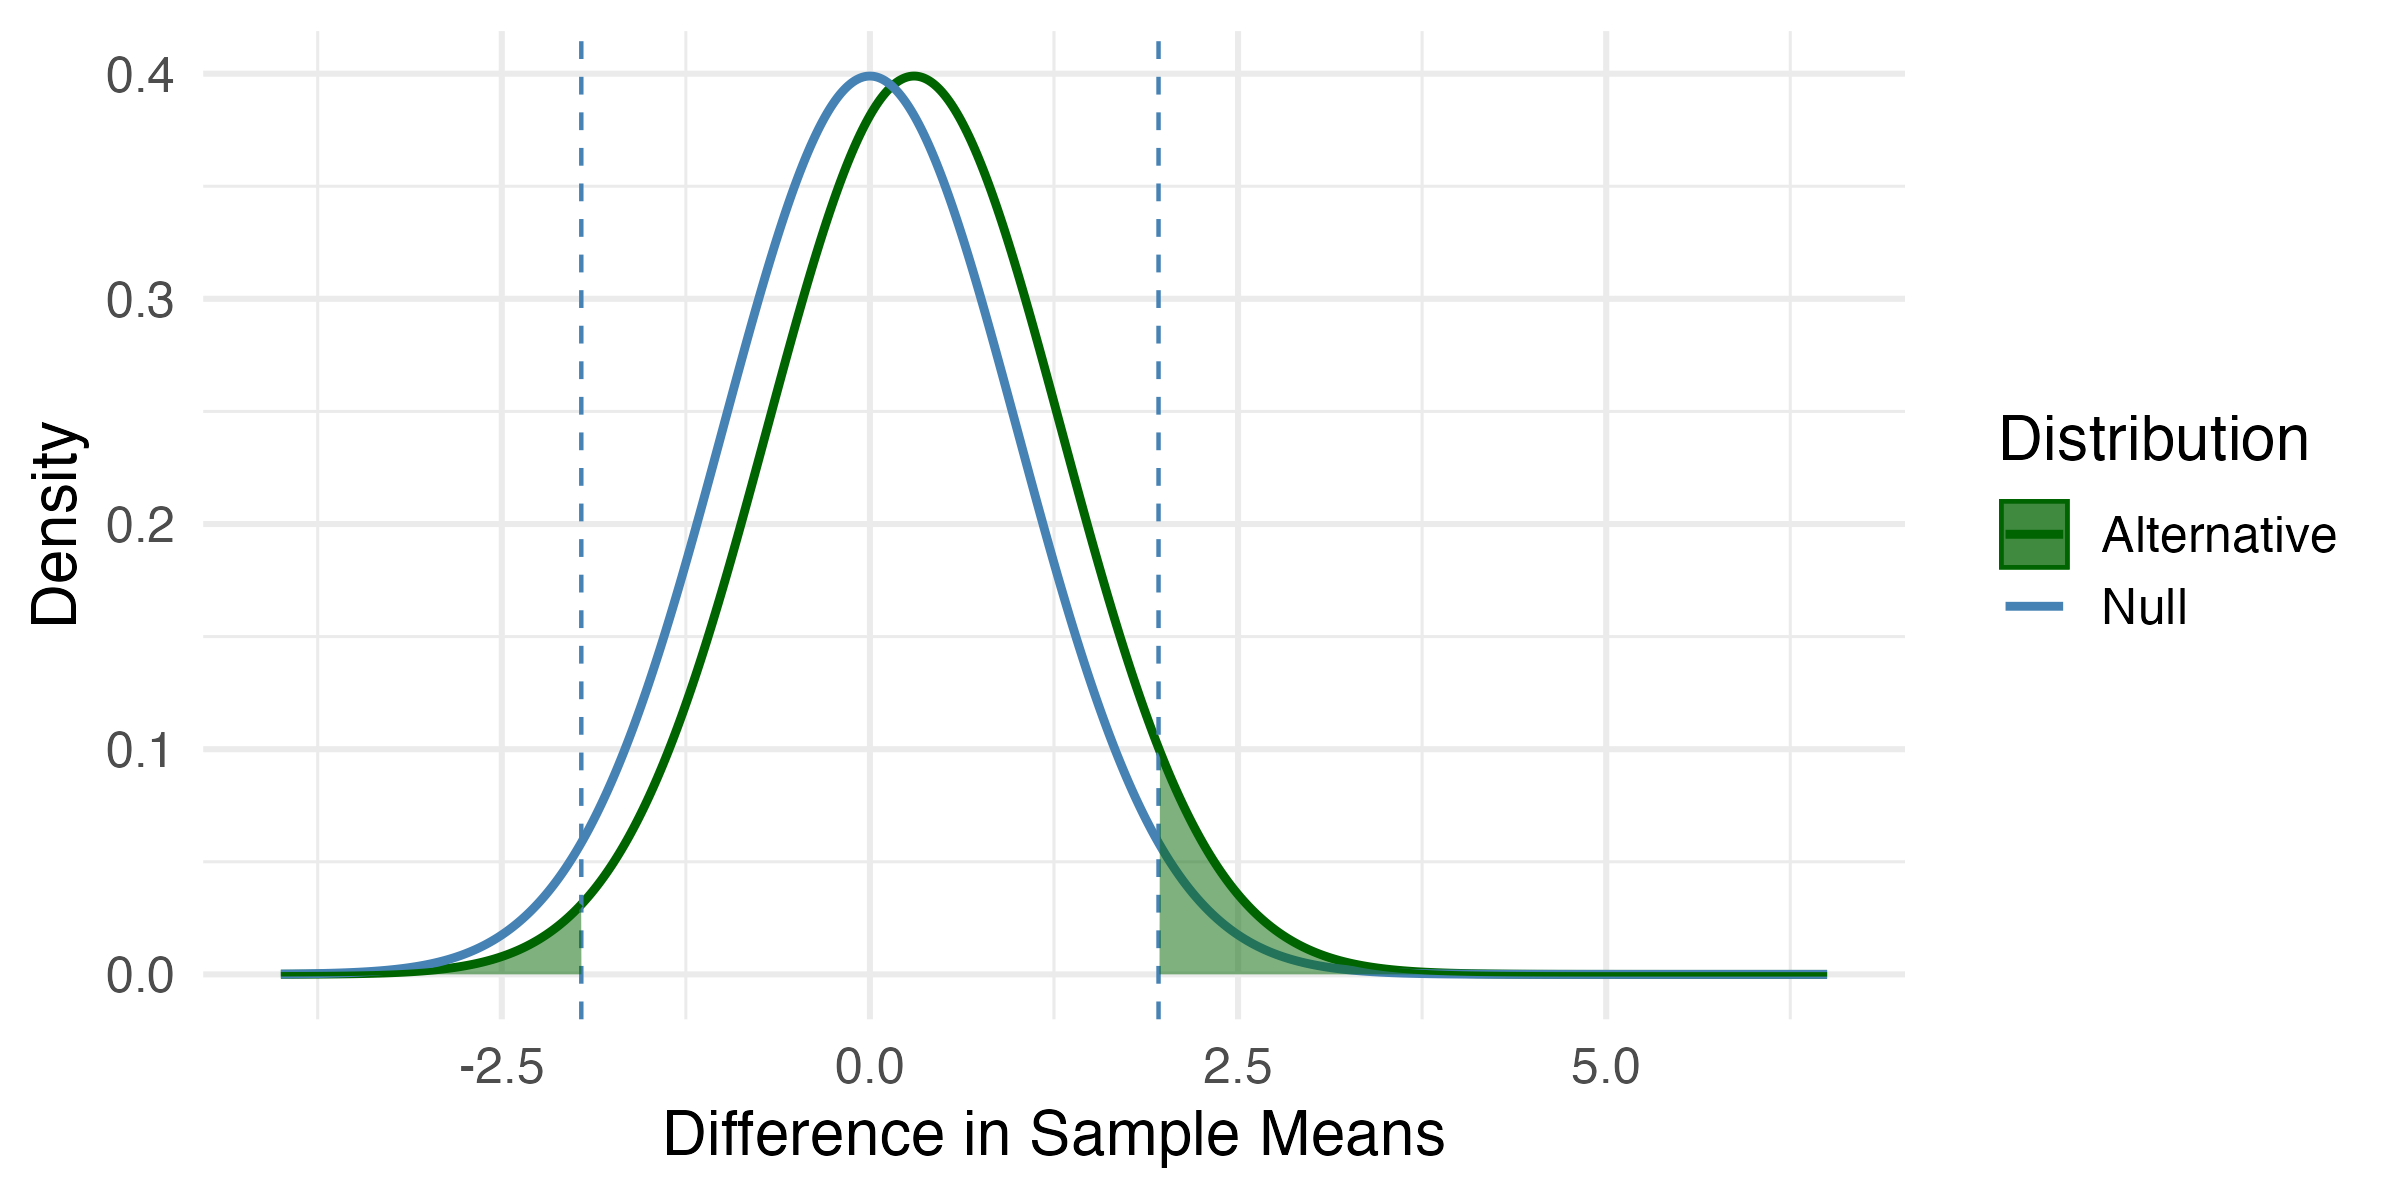
\includegraphics[width=\textwidth]{../Lecture27/figures/whatif_lowpower.png}
  \end{center}
  \small{
  \begin{enumerate}
	\item The probability of correctly rejecting $H_0$ is very low (\hl{Power})
	\item You can only detect large effects (leading to \hl{Magnitude Errors})
	\item It becomes possible to reject $H_0$ in the wrong direction (\hl{Sign Errors})
  \end{enumerate}
  }
\end{frame}

%%%%%%%%%%%%%%%%%%%%%%%%%%%%%%%%%%%%

\begin{frame}
	\frametitle{Retraction Watch: Thinking Fast and Slow}
	\begin{center}
		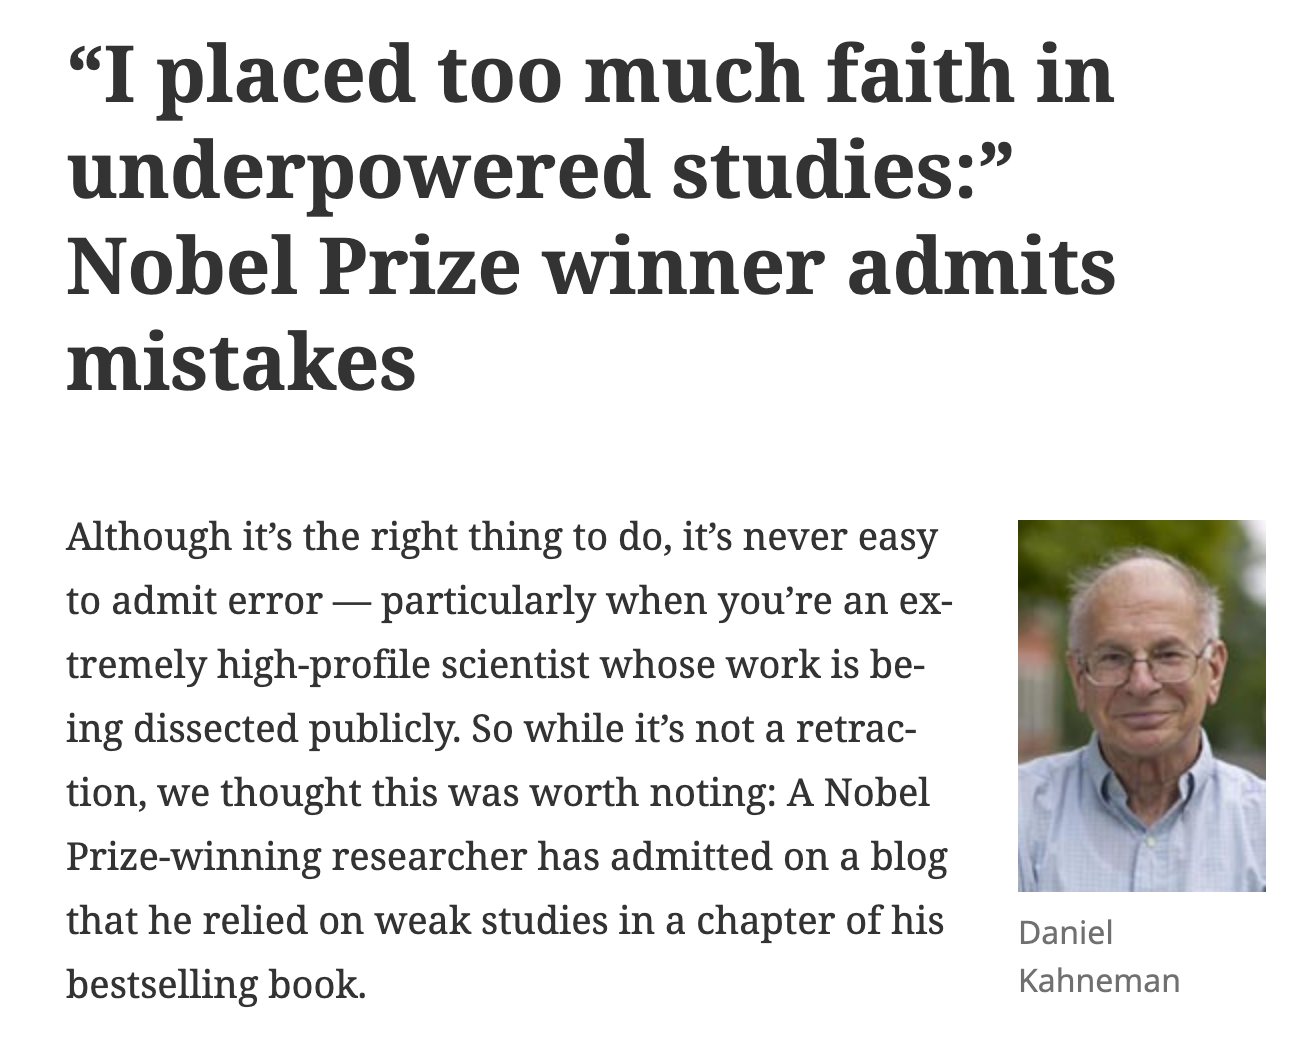
\includegraphics[height=0.75\textheight]{figures/Kahneman.png}
	\end{center}
	\soln{\footnotesize https://retractionwatch.com/2017/02/20/placed-much-faith-underpowered-studies-nobel-prize-winner-admits-mistakes/}
\end{frame}

%%%%%%%%%%%%%%%%%%%%%%%%%%%%%%%%%%%%

\begin{frame}
	\frametitle{The Replication Crisis in Science}
	\begin{itemize}
		\item Many published scientific findings fail to replicate when studies are repeated.
		\item John Ioannidis (2005): ``Why Most Published Research Findings Are False''
		\item Factors: small sample sizes, publication bias, p-hacking, selective reporting.
		\item Many of these issues relate to misuse of and overreliance on hypothesis testing.
	\end{itemize}
	\vspace{1em}
	\soln{\footnotesize Ioannidis, J.P.A. (2005). Why Most Published Research Findings Are False. PLoS Med 2(8): e124.}
\end{frame}

%%%%%%%%%%%%%%%%%%%%%%%%%%%%%%%%%%%%
% Beauty and Sex Ratios Example
%%%%%%%%%%%%%%%%%%%%%%%%%%%%%%%%%%%%
\begin{frame}
	\begin{center}
		
\includegraphics[height=0.75\textheight]{figures/Gelman.png}
	\end{center}
	\soln{\footnotesize Gelman, A., \& Carlin, J. (2014). Beyond Power Calculations. Perspectives on Psychological Science, 9(6), 641-651.}
\end{frame}


\section{Case Study: Beauty and Sex Ratios}

\begin{frame}

	\frametitle{Case Study: Beauty and Sex Ratios}

	\begin{columns}
		\column{0.55\textwidth}
			\textbf{Claim:} beautiful people are \textcolor{red}{8\%} more likely to have female offspring
			\begin{itemize}
				\item \textbf{N=2972} survey respondents
				\item Rated 1-5 on ``attractiveness''
				\item Recorded the sex of their first child
				\begin{itemize}
					\item Most attractive (5) had 56\% girls
					\item Others (1-4) had 48\% girls
				\end{itemize}
			\end{itemize}
		\vspace{0.2em}
		\begin{block}{}
			\footnotesize
				\textcolor{green!60!black}{Realistic effect sizes for sex ratios are about \textcolor{red}{\textbf{1\%}} (This is a generous estimate based on the literature for changes in sex ratios due to parental age, birth order, etc.)}
		\end{block}
		\vspace{0.5em}
		\column{0.44\textwidth}
			\textbf{Hypothesis Test}
			\begin{itemize}
				\item Level $\alpha = 0.05$
				\item Normal approx. $np > 15$
				\item Target parameter: $d = p_5 - p_{1-4}$
				\item Test statistic: $\hat{d} = \hat{p}_5 - \hat{p}_{1-4}$
				\item $H_0: d = 0$
				\item $H_a: d \neq 0$
				\item Inference: reject $H_0$, p-value$=0.015<0.05$
			\end{itemize}
	\end{columns}

\end{frame}

%%%%%%%%%%%%%%%%%%%%%%%%%%%%%%%%%%%%

\begin{frame}
	\frametitle{What was the standard error of the test statistic $\hat{d}$?}

	\vspace{0.5em}
	\begin{align*}
	&\textbf{p-value:}\quad \Pr(|d| > \hat{d}\mid H_0) = 0.015 \\
	&\Pr(d > \hat{d}\mid H_0) = \frac{0.015}{2} = 0.0075 \\
	&\frac{\hat{d} - 0}{\hat{\sigma}_{\hat{d}}} = Z \sim N(0,1) \\
	&\Pr\left(Z > \frac{\hat{d}}{\hat{\sigma}_{\hat{d}}} \mid H_0\right) = 0.0075
	\end{align*}

	Using R, $\Pr(Z > 2.4) = 0.0075$

	\begin{align*}
	\frac{\hat{d}}{\hat{\sigma}_{\hat{d}}} = 2.4 \implies \hat{\sigma}_{\hat{d}} = \frac{8}{2.4} = \textcolor{red}{3.3\%}
	\end{align*}

\end{frame}

%%%%%%%%%%%%%%%%%%%%%%%%%%%%%%%%%%%%

\section{R demo: (Shiny App) What did the power figure look like for the case study?}

%%%%%%%%%%%%%%%%%%%%%%%%%%%%%%%%%%%%
\begin{frame}
	\frametitle{Think/Pair/Share: Sex Ratios}
	\begin{center}
		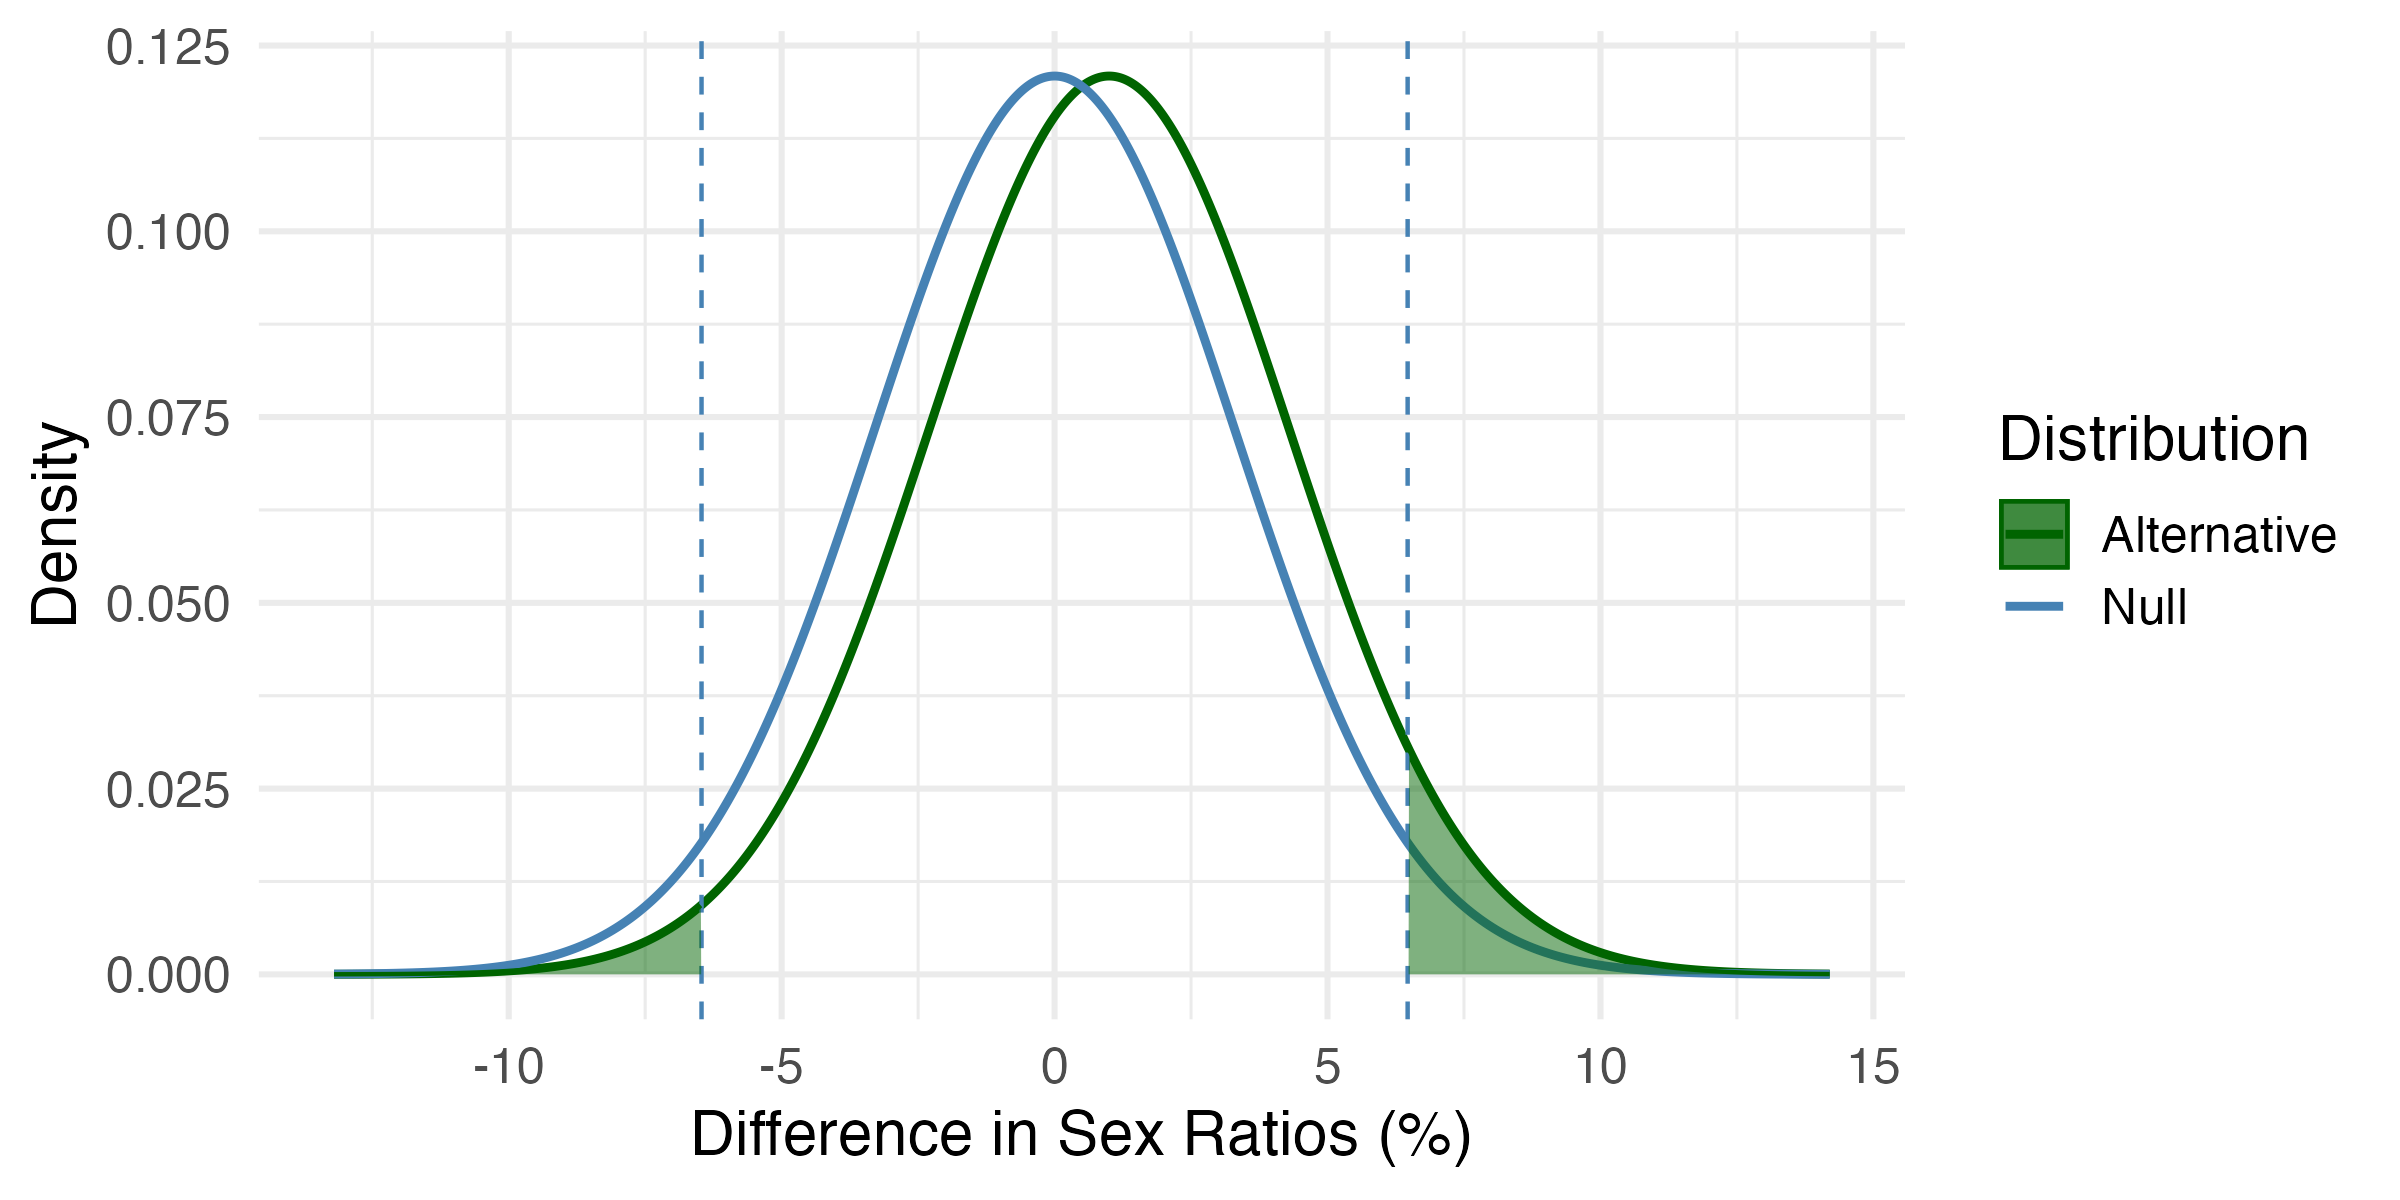
\includegraphics[height=0.5\textheight]{figures/whatif_sexratio.png}
	\end{center}
	\small{
	\begin{itemize}
		\item Approximately how big did the effect size have to be to reach significance?
		\item Approximately what was the power of the test to detect an effect of 1\%?
		\item What is the approximate probability that a statistically significant result is in the wrong direction (sign error)?
	\end{itemize}
	}
\end{frame}

%%%%%%%%%%%%%%%%%%%%%%%%%%%%%%%%%%%%

\solnGr{
\begin{frame}
	\frametitle{Think/Pair/Share: Sex Ratios}
	\begin{center}
		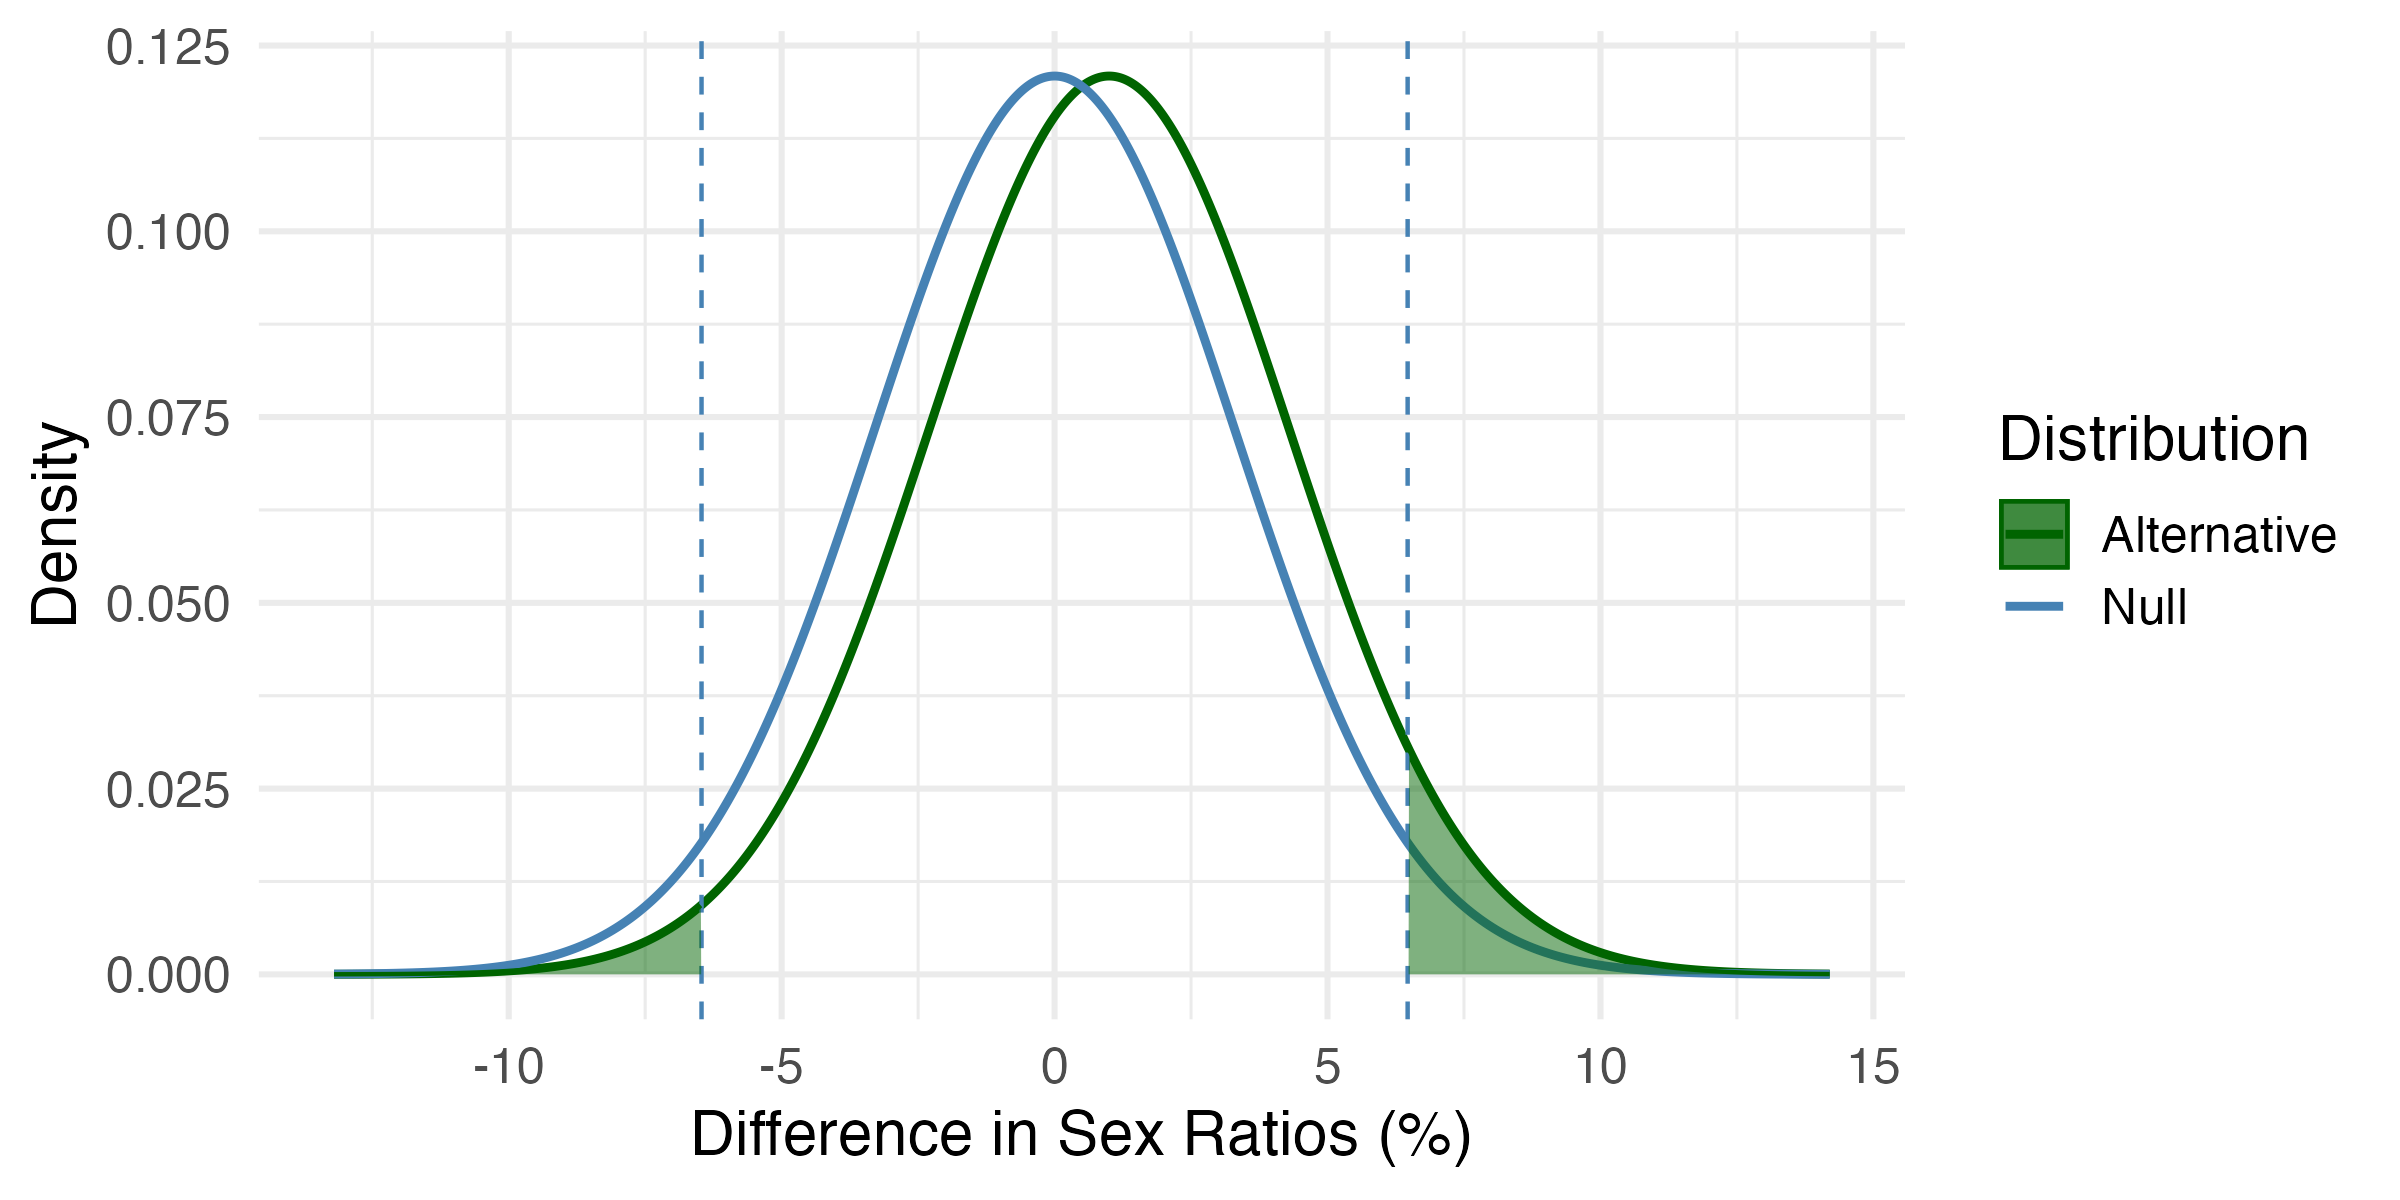
\includegraphics[height=0.4\textheight]{figures/whatif_sexratio.png}
	\end{center}
	\small{
	Based on this study design:
	\begin{itemize}
		\item The effect size had to be at least \hl{6.5\%} to reject the null hypothesis (but a realistic effect size would be less than 1\%)
		\item There was only a \hl{6\%} chance that the test could correctly reject the null hypothesis
		\item There was a \hl{20\%} chance that any significant result was in the wrong direction!
	\end{itemize}
	}
\end{frame}
}

%%%%%%%%%%%%%%%%%%%%%%%%%%%%%%%%%%%%

\begin{frame}
\frametitle{How many subjects would be required to detect an effect of 1\% with power 0.8?}
	Based on this study design:
	\begin{itemize}
		\item More than \hl{250,000 subjects} would be required to detect an effect of 1\% with power 0.8
	\end{itemize}
\end{frame}
	
%%%%%%%%%%%%%%%%%%%%%%%%%%%%%%%%%%%%
% Takeaways and Best Practices
%%%%%%%%%%%%%%%%%%%%%%%%%%%%%%%%%%%%
\section{Takeaways and Best Practices}
\begin{frame}
	\frametitle{Takeaways}
	\begin{itemize}
		\item Even if your sample size looks large, your power could be low if the population standard deviation is large or the effect size is small
		\item If your power is low and you reject the null hypothesis
		\begin{itemize}
			\item There is a high probability that your estimated effect is in the wrong direction (Sign Error)
			\item There is a high probability that your estimated effect is larger than any actual effect (Magnitude Error)
		\end{itemize}
	\end{itemize}
\end{frame}

\begin{frame}
	\frametitle{Best Practices}
	\begin{itemize}
		\item To avoid sign and magnitude errors, be sure to calculate power using a realistic effect size and only report results when power $>0.8$
		\begin{itemize}
			\item Never calculate power based on the effect size from the current experiment
			\item Avoid basing the effect size on prior studies with low power (due to small sample size or high standard deviation)
			\item Ideally, base it on prior studies with high power (even if the question of interest was different)
		\end{itemize}
		\item Consider power when designing studies and interpreting results
	\end{itemize}
\end{frame}


%%%%%%%%%%%%%%%%%%%%%%%%%%%%%%%%%%%%
% End document
%%%%%%%%%%%%%%%%%%%%%%%%%%%%%%%%%%%%

\end{document}